% !TeX program = xelatex
% disertasi.tex — Template XeLaTeX (versi bersih & rapi)
\documentclass[12pt,a4paper,oneside]{report}

% ---------------- Layout & Paket Dasar ----------------
\usepackage[a4paper, top=4cm, left=3cm, right=3cm, bottom=3cm]{geometry}
% \usepackage{showframe}    % untuk menampilkan margin (bisa dihapus nanti)
\usepackage{setspace}      % untuk kontrol spasi
\usepackage{titlesec}      % untuk atur ukuran heading
\usepackage{float}         % untuk kontrol posisi gambar/tabel
% Reduce top space before chapter title
\titlespacing*{\chapter}{0pt}{-20pt}{20pt}
\usepackage{graphicx}      % untuk gambar
\usepackage{listings}      % untuk "Daftar Tampilan" (kode/program)
\usepackage{caption}       % kontrol caption
\usepackage{indentfirst}   % ✅ buat paragraf pertama setiap bab ikut menjorok
\usepackage{ragged2e}      % ✅ menyediakan \justifying

% ---------------- Bahasa & Font (XeLaTeX) --------------
\usepackage{polyglossia}
\setmainlanguage{bahasai}  % ✅ gunakan bahasa Indonesia (tanpa warning)
\usepackage{fontspec}
\setmainfont{Times New Roman} % ganti ke TeX Gyre Termes bila TNR tidak tersedia

% ---------------- Penamaan elemen Indonesia ------------
\addto\captionsbahasai{%
  \renewcommand{\contentsname}{Daftar Isi}%
  \renewcommand{\listfigurename}{Daftar Gambar}%
  \renewcommand{\listtablename}{Daftar Tabel}%
  \renewcommand{\lstlistlistingname}{Daftar Tampilan}%
  \renewcommand{\abstractname}{Abstrak}%
}

% ---------------- Ukuran heading -----------------------
% Judul Bab = 14pt bold
\titleformat{\chapter}
  {\bfseries\fontsize{14pt}{16pt}\selectfont}
  {\thechapter}{1em}{}
% Subjudul (section, subsection) = 13pt bold
\titleformat{\section}
  {\bfseries\fontsize{13pt}{15pt}\selectfont}
  {\thesection}{1em}{}
\titleformat{\subsection}
  {\bfseries\fontsize{13pt}{15pt}\selectfont}
  {\thesubsection}{1em}{}

% ---------------- Bibliografi (spasi 1) ----------------
\usepackage[backend=biber,style=ieee,sorting=nyt,autolang=other]{biblatex}
\DeclareLanguageMapping{bahasa}{english}
\DeclareLanguageMapping{bahasai}{english}
% \addbibresource{references.bib}
% \AtBeginBibliography{\singlespacing}

% ---------------- Listings (Kode Program) -------------------
\usepackage{xcolor}
\usepackage{listings}

\lstdefinelanguage{PHP}{
  keywords={echo, array, if, else, elseif, function, return, class, public, private, protected, var, new},
  sensitive=true,
  comment=[l]{//},
  morecomment=[s]{/*}{*/},
  morestring=[b]",
}

\lstset{
  language=PHP,
  basicstyle=\ttfamily\small,
  keywordstyle=\color{blue}\bfseries,
  stringstyle=\color{red},
  commentstyle=\color{gray}\itshape,
  numbers=left,
  numberstyle=\tiny\color{gray},
  numbersep=8pt,
  tabsize=2,
  showstringspaces=false,
  breaklines=true,
  frame=single,
  captionpos=b,
}

% =======================================================
\begin{document}

  % ===================== HALAMAN JUDUL (spasi 1) =====================
  \begin{titlepage}
      \thispagestyle{empty}
      \begin{center}
          \Large{\textbf{ANALISIS ALGORITHMA DAN PENGEMBANGAN PERANGKAT LUNAK}}\\[0.5cm]
          \Large{\textbf{TUGAS KULIAH}}\\[0.5cm]

          \large{\textbf{disusun oleh}}\\
          \large{\textbf{Markani}}\\
          \large{\textbf{25201201010}}\\[2cm]

          
\includegraphics[width=5cm]{lambang-unitama-512-512.png}\\[1.5cm]

          \large{\textbf{PROGRAM STUDI MAGISTER ILMU KOMPUTER}}\\
          \large{\textbf{UNIVERSITAS TEKNOLOGI AKBA}}\\
          \large{\textbf{MAKASSAR}}\\
          \large{\textbf{2025}}\\
      \end{center}
  \end{titlepage}
  % ===================== TEKS UTAMA (spasi 1.5) ======================
  \onehalfspacing
  \justifying
  \chapter{Pendahuluan}
    Tugas Kuliah disusun sesuai dengan arahan yang diberikan oleh dosen pemateri perkuliahan, dimana tugas yang diberikan sebagai berikut
    \begin{enumerate}
      \item Memilih dua dari beberapa algoritma pengurutan terkecuali insertion sort.
      \item menimplementasikan algoritma tersebut dalam sebuah bahasa pemrograman tanpa menggunakan library yang sudah ada.
      \item Melakukan analisis terhadap algoritma yang telah diimplementasikan. dengan cara mengukur waktu eksekusi dari algoritma tersebut pada berbagai ukuran data yang berbeda (1000, 10000, 50000). 
      \item mencatat hasil tersebut kedalam tabel
    \end{enumerate}
    \par
      penulis menggunakan bahasa pemograman php 8.4 untuk mengimplementasikan algoritma pengurutan yang telah dipilih yaitu insertion sort dan quick sort.
      dan penulis telah menyimpan kode program pada repository github dengan alamat \\ \url{https://github.com/markaniph5/markani_s2_unitama} \\dimana hal ini bertujuan untuk memudahkan dosen pemateri dalam melakukan review terhadap kode program yang telah diimplementasikan dan mengikuti etika penelitian yaitu reproduceable.
      untuk menguji algoritma yang telah diimplementasikan penulis menggunakan data acak dengan berbagai ukuran data yaitu 1000, 10000, dan 50000. menggunakan PHP unit Testing untuk mengukur waktu eksekusi dari algoritma yang telah diimplementasikan.
      perangkat keras yang penulis gunakan untuk menguji algoritma yang telah diimplementasikan adalah sebagai berikut :
      \begin{figure}[H]
          \centering
          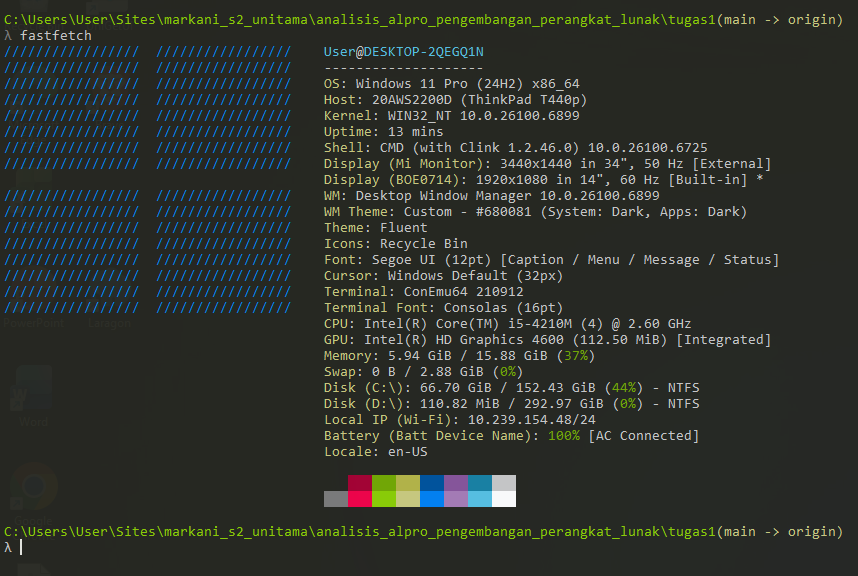
\includegraphics[width=1\linewidth]{hardware.png}
          \caption*{Spesifikasi Perangkat Keras}
      \end{figure}
  \chapter{Pembahasan}
    \section{Algoritma Pengurutan}
      Algoritma pengurutan adalah metode atau prosedur yang digunakan untuk mengatur elemen- elemen dalam suatu kumpulan data sehingga mereka berada dalam urutan tertentu.
      Urutan ini bisa berdasarkan nilai numerik, abjad, atau kriteria lainnya. Algoritma pengurutan sangat penting dalam ilmu komputer karena mereka digunakan dalam berbagai aplikasi,
      mulai dari pengolahan data hingga pencarian informasi. ada pun algorithma yang penulis pilih adalah sebagai berikut :
      \begin{lstlisting}
        <?php
          declare(strict_types=1);
          namespace Markani\Tugas1\App;

          class Algorithm {
              public function quickSort(array $arr): array {
                  $n = count($arr);
                  if ($n <= 1) {
                      return $arr;
                  }

                  // choose pivot (middle element)
                  $pivot = $arr[intdiv($n, 2)];

                  $left = [];
                  $equal = [];
                  $right = [];

                  foreach ($arr as $value) {
                      if ($value < $pivot) {
                          $left[] = $value;
                      } elseif ($value > $pivot) {
                          $right[] = $value;
                      } else {
                          $equal[] = $value;
                      }
                  }

                  return array_merge($this->quickSort($left), $equal, $this->quickSort($right));
              }

              public function insertionSort(array $arr): array {
                  $n = count($arr);
                  for ($i = 1; $i < $n; $i++) {
                      $key = $arr[$i];
                      $j = $i - 1;
                      while ($j >= 0 && $arr[$j] > $key) {
                          $arr[$j + 1] = $arr[$j];
                          $j--;
                      }
                      $arr[$j + 1] = $key;
                  }
                  return $arr;
              }
          }
      \end{lstlisting}
    \section{Kode Pengujian}
      Kode pengujian yang penulis gunakan untuk mengukur waktu eksekusi dari algorithma yang telah diimplementasikan adalah sebagai berikut :
      \begin{lstlisting}
        <?php
          declare(strict_types=1);
          use PHPUnit\Framework\TestCase;
          use Markani\Tugas1\App\Algorithm;

          final class InsertionShort1000DataTest extends TestCase
          {

              public function testAlgoithmInsertionSortFirstCase(): void
              {
                  // generate 1000 data
                  $total_data = 1000;
                  $data = [];
                  for ($i = 0; $i < $total_data; $i++ ) {
                      $data[] = $i+1;
                  }
                  $test_data = $data;
                  shuffle($test_data);

                  // mendeklarasikan objek
                  $algorithm = new Algorithm();
                  $sorted_data = $algorithm->insertionSort($test_data);
                  $this->assertEquals($data[$total_data - 1], $sorted_data[$total_data - 1]);
              }
          }
      \end{lstlisting}

      \begin{lstlisting}
        <?php
          declare(strict_types=1);
          use PHPUnit\Framework\TestCase;
          use Markani\Tugas1\App\Algorithm;

          final class InsertionShort10000DataTest extends TestCase
          {

            public function testAlgoithmInsertionSortSecondCase(): void
            {
                // generate data
                $total_data = 10000;
                $data = [];
                for ($i = 0; $i < $total_data; $i++ ) {
                    $data[] = $i+1;
                }
                $test_data = $data;
                shuffle($test_data);

                // mendeklarasikan objek
                $algorithm = new Algorithm();
                $sorted_data = $algorithm->insertionSort($test_data);
                $this->assertEquals($data[$total_data - 1], $sorted_data[$total_data - 1]);
            }
          }
      \end{lstlisting}

      \begin{lstlisting}
        <?php
          declare(strict_types=1);
          use PHPUnit\Framework\TestCase;
          use Markani\Tugas1\App\Algorithm;

          final class InsertionShort50000DataTest extends TestCase
          {

              public function testAlgoithmInsertionSortThirdCase(): void
              {
                  // generate data
                  $total_data = 50000;
                  $data = [];
                  for ($i = 0; $i < $total_data; $i++ ) {
                      $data[] = $i+1;
                  }
                  $test_data = $data;
                  shuffle($test_data);

                  // mendeklarasikan objek
                  $algorithm = new Algorithm();
                  $sorted_data = $algorithm->insertionSort($test_data);
                  $this->assertEquals($data[$total_data - 1], $sorted_data[$total_data - 1]);
              }
          }
      \end{lstlisting}

      \begin{lstlisting}
        <?php
          declare(strict_types=1);
          use PHPUnit\Framework\TestCase;
          use Markani\Tugas1\App\Algorithm;

          final class QuickShort1000DataTest extends TestCase
          {

              public function testAlgoithmQuickSortFirstCase(): void
              {
                  // generate 1000 data
                  $total_data = 1000;
                  $data = [];
                  for ($i = 0; $i < $total_data; $i++ ) {
                      $data[] = $i+1;
                  }
                  $test_data = $data;
                  shuffle($test_data);

                  // mendeklarasikan objek
                  $algorithm = new Algorithm();
                  $sorted_data = $algorithm->quickSort($test_data);
                  $this->assertEquals($data[$total_data - 1], $sorted_data[$total_data - 1]);
              }
          }
      \end{lstlisting}

      \begin{lstlisting}
        <?php
          declare(strict_types=1);
          use PHPUnit\Framework\TestCase;
          use Markani\Tugas1\App\Algorithm;

          final class QuickShort10000DataTest extends TestCase
          {

              public function testAlgoithmQuickSortSecondCase(): void
              {
                  // generate data
                  $total_data = 10000;
                  $data = [];
                  for ($i = 0; $i < $total_data; $i++ ) {
                      $data[] = $i+1;
                  }
                  $test_data = $data;
                  shuffle($test_data);

                  // mendeklarasikan objek
                  $algorithm = new Algorithm();
                  $sorted_data = $algorithm->quickSort($test_data);
                  $this->assertEquals($data[$total_data - 1], $sorted_data[$total_data - 1]);
              }
          }
      \end{lstlisting}

      \begin{lstlisting}
        <?php
          declare(strict_types=1);
          use PHPUnit\Framework\TestCase;
          use Markani\Tugas1\App\Algorithm;

          final class QuickShort50000DataTest extends TestCase
          {
              public function testAlgoithmQuickSortThirdCase(): void
              {
                  // generate data
                  $total_data = 50000;
                  $data = [];
                  for ($i = 0; $i < $total_data; $i++ ) {
                      $data[] = $i+1;
                  }
                  $test_data = $data;
                  shuffle($test_data);

                  // mendeklarasikan objek
                  $algorithm = new Algorithm();
                  $sorted_data = $algorithm->quickSort($test_data);
                  $this->assertEquals($data[$total_data - 1], $sorted_data[$total_data - 1]);
              }
          }
      \end{lstlisting}
    
    \section{Luaran Pengujian}
      luaran hasil pengujian dari kode pengujian yang telah penulis lakukan adalah sebagai berikut :
      \begin{figure}[H]
          \centering
          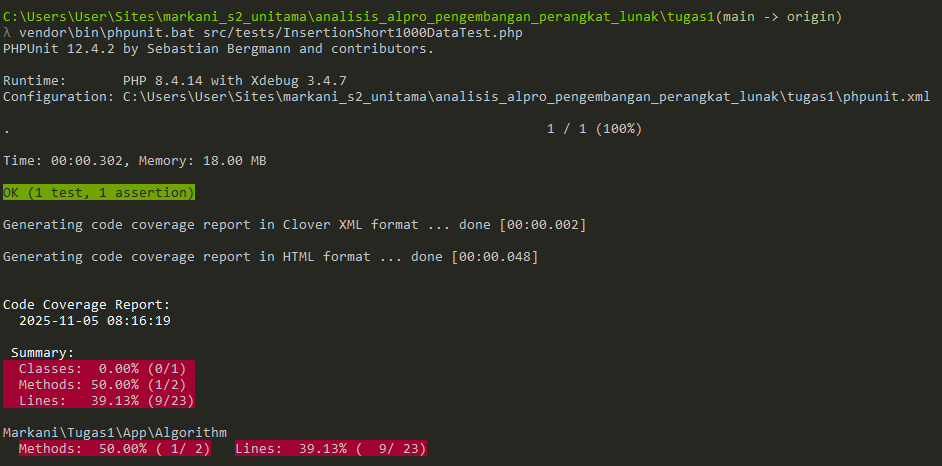
\includegraphics[width=1\linewidth]{insertion_sort_1.png}
          \caption*{Insertion Sort 1000 Data}
      \end{figure}   
      
      \begin{figure}[H]
          \centering
          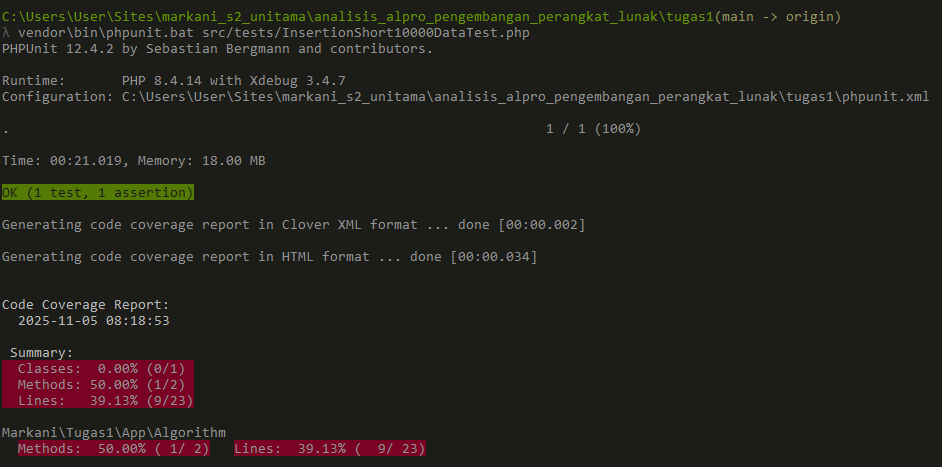
\includegraphics[width=1\linewidth]{insertion_sort_2.png}
          \caption*{Insertion Sort 10000 Data}
      \end{figure}
\end{document}
